% Resource util maps
\begin{figure}[t]
  \centering
  \begin{subfigure}[t]{0.5\columnwidth}
    \centering
    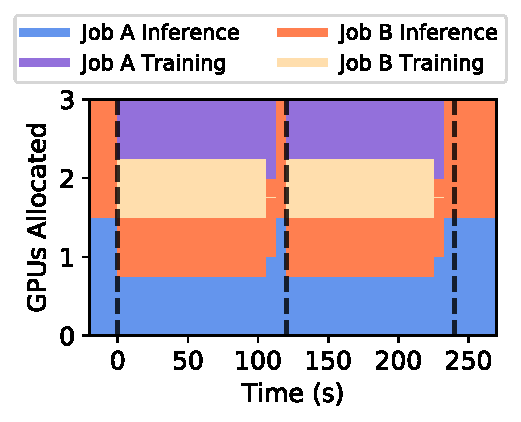
\includegraphics[width=\linewidth]{figures/motivation/Scheduler/schedmot_res_eventual_best_cfgs.pdf}
    \caption{\small Naive, eventual best cfgs}
    \label{fig:schedmot-res-naive}
  \end{subfigure}  
%  ~~
%  \begin{subfigure}[t]{0.3\linewidth}
%    \centering
%    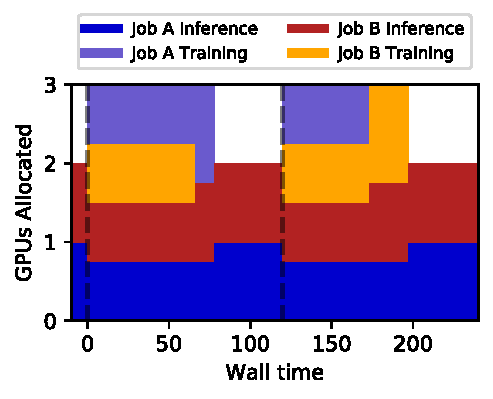
\includegraphics[width=\linewidth]{figures/motivation/Scheduler/schedmot_res_optimal_cfgs.pdf}
%    \caption{\small Optimal cfgs for retraining window}
%    \label{fig:schedmot-res-optimalcfg}
%  \end{subfigure}
  ~~
  \begin{subfigure}[t]{0.5\columnwidth}
    \centering
    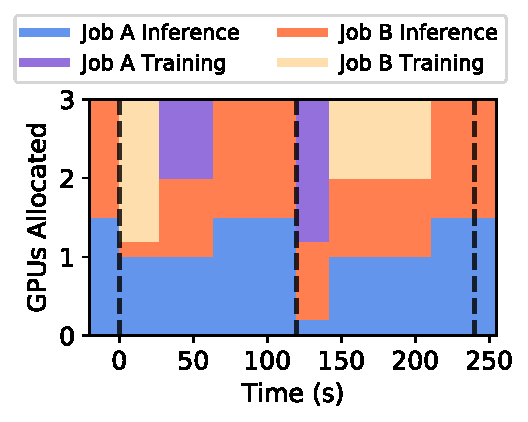
\includegraphics[width=\linewidth]{figures/motivation/Scheduler/schedmot_res_prioritization_and_optimal_cfgs.pdf}
    \caption{\small Optimal cfgs with prioritization}
    \label{fig:schedmot-res-prioritization}
  \end{subfigure}
  ~~
  \caption{\bf\small Resource allocation maps for toy retraining schedules in Figure \ref{fig:schedmot}. (\ref{fig:schedmot-naive}) and (\ref{fig:schedmot-res-optimalcfg}) run a fair scheduler which evenly splits resources between the two cameras. (\ref{fig:schedmot-res-prioritization}) deprioritizes Camera B's inference task due because of its low accuracy, and instead focuses resources on retraining it. On the other hand, Camera A's inference job is already at an high accuracy, thus it deprioritizes it's retraining job until Camera B is retrained. \ga{Unused GPUs when retraining is not happening; can we fix it?}}
  \label{fig:schedmot-res}
\end{figure}


\subsection{Checkpointing Models}
\label{subsec:checkpoint}
In the process of retraining, the inference accuracy increases only when the model being retrained is loaded into the inference job's memory. This checkpointing has both, a benefit (the accuracy improvement is available faster, thus mean inference accuracy increases) and a cost (cost of checkpointing model and loading into memory). Thus, the frequency of checkpointing is a careful decision dependent on the expected gain in accuracy and the cost of checkpointing.  \romil{Add figure like Fig 5b, except with more frequent checkpointing to show smooth increase and overall higher accuracy.}

\textbf{How do we do checkpointing?} Ekya carefully evaluates the cost-benefit of checkpointing to arrive at the optimal checkpointing rate. The cost is defined as the amount of time it takes to checkpoint a model in memory and reload it into the inference model. The benefit of checkpointing is the higher accuracy that will available for the remainder of the retraining period.

\textbf{Measuring the cost ($\delta$): } The time taken to checkpoint a model and load it is dependent on the size of the model. While the model is being checkpointed, the model training must be halted \romilc{Should it?}. Since the model size and architecture does not change over retraining windows, it is possible to profile the checkpoint cost beforehand. In our experiments \romilc{TODO}, we found that checkpointing requires \romilc{xx} seconds and restoring requires \romilc{yy} seconds, creating a total cost of \romilc{$\delta$} seconds on the checkpointing 

\textbf{Measuring the benefit (accuracy improvement): } Consider a single video stream with a single retraining job and a single inference job. Let $\tau$ be the time taken by the retraining job to complete. At any time instant $t$ since the start of the retraining window, let the inference accuracy of the job be $a$. The remaining amount of time in the window can be calculated as $T-t$, where $T$ is the length of the retraining window and $A$ is the final retrained accuracy. Without checkpointing, the mean inference accuracy in the remainder retraining window is \romil{Change to integral}:

\[
    base\_acc = \frac{(\tau-t)*a + (T-\tau)*A}{T} 
\]

With checkpointing (\romilc{Figure xx}), \name{} must decide if at every timestep $t$ the model must be checkpointed. By checkpointing, the inference accuracy improves while the retraining is still running, but a checkpoint also increases the total train time by $\delta$. Assume the inference accuracy at start is $a$ and increases to $a^{*}$ Thus the inference accuracy if checkpointed at time $t$ is:  \romil{Careful, this is validation accuracy.. maybe include a validation->test acc conversion facor?}
\[
    acc = \frac{(\tau-t)*a^{*} + (T-\tau-\delta)*A}{T} 
\]

\textbf{Checkpointing Decision} Thus, models must be checkpointed only when $acc > base\_acc$, and this decision is evaluated at every time instant $t$. Whenever this statment is true at the current $t$, the model is checkpointed.

